\setcounter{chapter}{3}
\chapter{Hiện thực và triển khai}

\section{Kiến trúc của EHAT}

\begin{center}
	\begin{figure}[htp]
		\begin{center}
			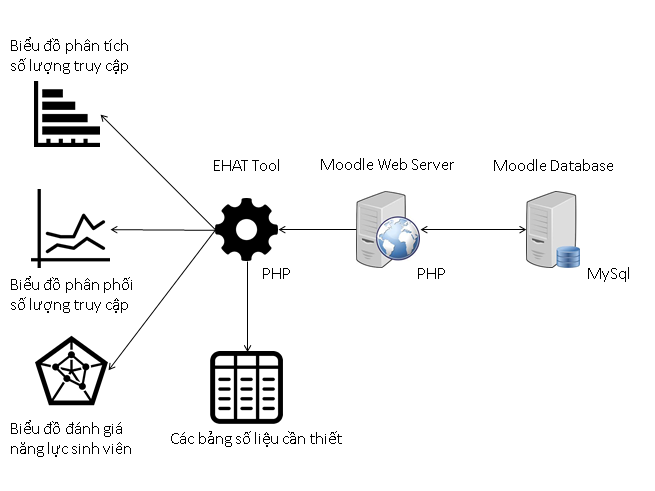
\includegraphics[scale=1]{img/kientrucehat}
		\end{center}
		\caption{Kiến trúc hệ thống EHAT}
		\label{refhinh21}
	\end{figure}
\end{center}

Trên đây là kiến trúc của EHAT trong Moodle. Tiếp đến chúng ta sẽ cùng đi tìm hiểu cách để hiện thực những chức năng của EHAT mà nhóm đã xây dựng.

\section{Hiện thực những chức năng của EHAT}

EHAT là công cụ dễ dàng để sử dụng giúp người dùng phân tích được những dữ liệu trong một khóa học trực tuyến. Bên cạnh đó EHAT còn hỗ trợ cho HV trong quá trình học tập trực tuyến.

Công cụ EHAT hiện nay sẽ hỗ trợ tổng cộng 5 chức năng chính, trong đó 4 chức năng sẽ dành cho GV còn 1 chức năng là của HV. Trước tiên chúng ta sẽ cùng tìm hiểu về 4 chức năng mà EHAT cung cấp cho GV.

\subsection{Đối với GV}

EHAT sẽ cung cấp năm chức năng chính đối với GV như hình sau:

\begin{center}
	\begin{figure}[htp]
		\begin{center}
			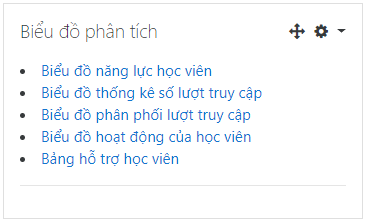
\includegraphics[scale=1]{img/gvtool}
		\end{center}
		\caption{Bốn chức năng mà EHAT mang lại cho GV}
		\label{refhinh27}
	\end{figure}
\end{center}

Trên đây là hình ảnh minh họa năm chức năng mà EHAT mang lại cho GV, tiếp theo chúng ta sẽ cùng đi vào chi tiết từng chức năng trên xem chúng có gì hay.

Để thực hiện các chức năng này nhóm đã có tham khảo một phần mã nguồn ở \cite{code} nhằm lấy dữ liệu từ log file để vẽ biểu đồ chính xác hơn

\subsubsection{Biểu đồ đánh giá năng lực học viên}
\begin{itemize}
	\item Chức năng đầu tiên mà EHAT giành cho GV đó là chức năng đánh giá năng lực học viên. Ở chức năng này EHAT sẽ sử dụng biểu đồ mạng nhện (Spider web) để mô tả năng lực của từng cá nhân HV. Kết quả sẽ chỉ ra số điểm trung bình của các tiêu chí mà GV thiết lập để đánh giá. Bên cạnh đó còn có thêm chức năng so sánh năng lực của hai HV để thấy rõ sự khác biệt về năng lực mỗi cá nhân trong khóa học.
	
	\item Để hiện thực chức năng này nhóm đã sử dụng dữ liệu về điểm số các bài kiểm tra của học viên được thu thập từ bảng mdl\_quiz\_grades trong cơ sở dữ liệu của Moodle đồng thời kết hợp với giá trị đầu vào như id của học viên, id của các bài kiểm tra,... từ đó ta tính trung bình để tìm ra được số điểm của một tiêu chí cần mô tả. Đồng thời kết hợp với biểu đồ mạng nhện được hỗ trợ bởi thư viện Highcharts để đưa giá trị ấy về dạng trực quan dễ tham khảo hơn.
\end{itemize}

\subsubsection{Biểu đồ thống kê số lượt truy cập}
\begin{itemize}
	\item Để sử dụng chức năng này đầu tiên người dùng phải chọn hạng mục mà mình muốn phân tích số liệu. Ví dụ về các hạng mục mà EHAT hỗ trợ người dùng phân tích:
	
	\begin{itemize}
		\item Bài tập lớn (Assignment)
		\item Trò chuyện (Chat)
		\item Lựa chọn (Choice)
		\item Phản hồi (Feedback)
		\item Diễn đàn (Forum)
		\item Bài giảng (Lesson)
		\item Câu hỏi (Quiz)
		\item Gói SCORM
		\item Khảo sát (Survey)
		\item Wiki
		\item Hội thảo (Workshop)
		\item Sách (Book)
		\item Tài nguyên (Resource)
		\item Tệp tin (Folder)
		\item Trang (Page)
		\item Đường dẫn (URL)
	\end{itemize}

	\item Chức năng này cho phép người dùng xem số lượt học viên truy cập và không truy cập của từng hạng mục cụ thể mà mình muốn phân tích. Chức năng này giúp GV thấy được mức độ hiệu quả của các tài nguyên trong khóa học để từ đó có những điều chình phù hợp cho khóa học của mình.
	
	\item Chức năng này nhóm đã đọc log file được lưu trữ trong bảng mdl\_logstore\_standard\_log của Moodle để đếm số lượng truy cập vào một mô-đun, một mô-đun được truy cập khi mô-đun đó có thể hiện hành động "viewed" hoặc "submission" được mô tả ở cột "action" và cột "instance" sẽ là cột mô tả id của mô-đun mà ta muốn tham khảo. Kèm với việc sử dụng biểu đồ cột ngang để mô tả chính xác những dữ liệu mà nhóm thu thập được.
\end{itemize}

\subsubsection{Biểu đồ phân phối lượt truy cập}
\begin{itemize}
	\item Chức năng sẽ hiển thị cho người dùng một bảng số liệu chứa những thông tin về:
	\begin{itemize}
		\item Số lần HV truy cập vào khóa học
		\item Số ngày mà HV truy cập theo tuần kèm biểu đồ mô tả
		\item Biểu đồ phần trăm lượt truy cập kèm theo đó là biểu đồ thể hiện chi tiết số lần truy cập của học viên
	\end{itemize}
	
	\item Bên cạnh đó bảng số liệu cũng có kèm theo dấu hiệu cho thấy HV có thường xuyên truy cập vào khóa học hay không. Để hiện thực được chức năng này ta cần lấy ra được những giá trị như sau:
	
	\begin{itemize}
		\item Số lượng ngày được truy cập trong một tuần. Dữ liệu này ta cũng sử dụng dữ liệu từ bảng mdl\_logstore\_standard\_log với điều kiện hành động của học viên là "viewed" và mục tiêu tác động đó là "course" và ta sẽ tính toán số tuần dựa vào ngày bắt đầu của khóa học đến thời điểm hiện tại.
		
		\item Lấy thông tin của tất cả các mô-đun được sử dụng trong khóa học thông qua bảng course\_modules của Moodle. Từ đó ta tiếp tục sử dụng bảng mdl\_logstore\_standard\_log để đếm số lần truy cập vào một mô-đun của một học viên đồng thời tính được số mô-đun mà học viên ấy truy cập và không truy cập.
	\end{itemize}
	
	Sau khi lấy được những dữ liệu như trên nhóm đã dùng bảng số liệu, biểu đồ đường, biểu đồ tròn, biểu đồ cột đứng để thể hiện các giá trị của những dữ liệu ấy.
	
\end{itemize}

\subsubsection{Biểu đồ hoạt động của học viên}
\begin{itemize}
	\item Biểu đồ này cũng đọc dữ liệu từ bảng mdl\_logstore\_standard\_log để thu thập thời gian hoạt động của từng học viên
	\item Bên cạnh đó biểu đồ có phân loại hai nhóm học viên như sau:
	\begin{itemize}
		\item Nhóm 1: Học viên hoạt động từ khung giờ 6:00 - 18:59
		\item Nhóm 2: Học viên hoạt động từ khung giờ 19:00 - 5:59
	\end{itemize}
	\item Tất cả dữ liệu thu được đều được mô tả dưới dạng biểu đồ trực quan.
\end{itemize}

\subsubsection{Bảng hỗ trợ học viên}
\begin{itemize}
	\item Chức năng cuối cùng mà EHAT hỗ trợ nhằm giúp cho GV thêm tài liệu tham khảo đối với mỗi câu hỏi trong mỗi bài kiểm tra. GV có thể thêm đoạn text hoặc một đường dẫn đến nơi mà mình muốn HV tham khảo. Nội dung sẽ được lưu trữ vào cơ sở dữ liệu và hiển thị cho học viên khi học viên sử dụng chức năng của EHAT.
	
	\item Chức năng này để xây dựng nhóm đã tạo thêm một bảng vào database của Moodle nhằm lưu trữ id của câu hỏi và nội dung tài liệu tham khảo. Bảng này sẽ tự động thêm vào Database khi ta thêm khối EHAT.
\end{itemize}

\subsection{Đối với HV}

Hiện nay EHAT chỉ cung cấp 1 chức năng cho học viên:

\subsubsection{Bảng xem lại khóa học}
\begin{itemize}
	\item EHAT hiện chỉ hỗ trợ cho HV chức năng xem lại toàn bộ bài các câu trả lời từ lần làm bài cuối cùng của mình. Trong đó sẽ chỉ rõ câu nào HV trả lời đúng và câu nào HV trả lời sai. Đi kèm với đó là nội dung chi tiết của từng câu hỏi và tài liệu tham khảo nhằm hỗ trợ HV học tập tốt hơn trong quá trình tự học của mình.
	
	\vskip 5cm
	\item Chức năng này nhóm đã lấy tất cả thông tin cần thiết của các bài kiểm tra trong lần làm bài cuối cùng của học viên và dữ liệu bên bảng mà nhóm đã tạo thêm để hiển thị. Tất cả thông tin ấy có trong các bảng sau:
	\begin{itemize}
		\item mdl\_quiz
		\item mdl\_question\_attempt\_steps 
		\item mdl\_question\_attempts
		\item mdl\_quiz\_grades
		\item mdl\_quiz\_slots
		\item mdl\_question
	\end{itemize}
\end{itemize}

\newpage
\section{Đặc tả yêu cầu hệ thống}

\subsection{Yêu cầu chung}

\begin{center}
	\begin{table}[!htp]
		\centering
		\begin{tabular}{|c|c|c|}
			\hline 
			STT & Nội dung & Chi tiết \\ 
			\hline 
			1 & Hệ điều hành & Ubuntu 16.04 \\ 
			\hline 
			2 & Database Server & MySQL  5.6/5.7 \\ 
			\hline 
			3 & Content Server & Apache, >= PHP 7, >= Moodle 3.6 \\ 
			\hline 
		\end{tabular} 
		\caption{Yêu cầu chung của hệ thống}
		\label{bang20}
	\end{table}
\end{center}

\subsection{EHAT đối với GV}
\subsubsection{Biểu đồ đánh giá năng lực học viên}
\begin{itemize}
	\item Giới thiệu: Giảng viên có thể đánh giá năng lực của từng cá nhân HV hoặc so sánh 2 HV với nhau.
	\item Đầu vào
	\begin{itemize}
		\item GV nhập vào số tiêu chí cần thiết lập và chọn nút "Thiết lập".
		\item GV nhập tên các tiêu chí và chọn dữ liệu cho chúng.
		\item GV chọn nút "So sánh" nếu muốn so sánh 2 HV với nhau.
		\item Chọn HV cần phân tích.
		\item Nhấn nút "Xác nhận" để xem biểu đồ.
	\end{itemize}
	\item Quy trình thực hiện
	\begin{itemize}
		\item GV nhấn chọn "Biểu đồ năng lực học viên" từ giao diện của Khối EHAT.
		\item GV nhập vào số tiêu chí cần thiết lập và chọn nút "Thiết lập".
		\item GV nhập tên các tiêu chí và chọn dữ liệu cho chúng.
		\item GV chọn nút "So sánh" nếu muốn so sánh 2 HV với nhau.
		\item Chọn HV cần phân tích.
		\item Nhấn nút "Xác nhận" để xem biểu đồ.
	\end{itemize}
	\item Đầu ra: Giao diện sẽ hiển thị biểu đồ mạng nhện thể hiện năng lực của một học viên hoặc so sánh 2 học viên mà ta đã chọn để phân tích ở trên.
	\item Xủ lí lỗi
	\begin{itemize}
		\item Nếu GV nhập số tiêu chí ít hơn 3 thì sẽ hiển thị thông báo lỗi và yêu cầu GV nhập lại.
		\item Nếu tên các tiêu chí hoặc dữ liệu của chúng chưa được thêm thì sẽ hiển thị thông báo yêu cầu GV nhập.
		\item Nếu hai HV so sánh là như nhau thì sẽ hiển thị thông báo lỗi.
	\end{itemize}
\end{itemize}

\subsubsection{Biểu đồ thống kê số lượt truy cập}
\begin{itemize}
	\item Giới thiệu: Giảng viên sử dụng biểu đồ để quan sát số lượng HV tương tác với một hạng mục trong khóa học.
	\item Đầu vào
	\begin{itemize}
		\item Chọn hạng mục cần tham khảo (Có thể nhấn nút chọn tất cả để xem hết tất cả các hạng mục).
		\item Thiết lập thời gian bắt đầu.
		\item Nhấn nút "Xem biểu đồ" để hiển thị kết quả.
	\end{itemize}
	\item Quy trình thực hiện
	\begin{itemize}
		\item GV nhấn chọn "Biểu đồ thống kê số lượt truy cập" từ giao diện của Khối EHAT
		\item GV sẽ chọn hạng mục cần tham khảo (Có thể nhấn nút chọn tất cả để xem hết tất cả các hạng mục).
		\item GV thiết lập thời gian bắt đầu (Thời gian mặc định là ngày khóa học bắt đầu).
		\item Nhấn nút "Xem biểu đồ" để hiển thị kết quả.
	\end{itemize}
	\item Đầu ra: Giao diện sẽ hiển thị biểu đồ cột ngang thể hiện tất cả số lượt truy cập và không truy cập của HV đối với từng hạng mục mà ta đã chọn. Đồng thời hiển thị thêm chi tiết HV nào truy cập hay không truy cập trong hạng mục đó.
	\item Xủ lí lỗi
	\begin{itemize}
		\item Nếu GV không chọn hạng mục thì sẽ hiển thị thông báo lỗi.
	\end{itemize}
\end{itemize}
\subsubsection{Biểu đồ phân phối lượt truy cập}
\begin{itemize}
	\item Giới thiệu: GV dùng để xem xét chi tiết mức độ tương tác của từng cá nhân HV đối với các tài nguyên trong quá trình học.
	\item Đầu vào: 
	\begin{itemize}
		\item Chọn mục "Biểu đồ phân phối lượt truy cập" từ giao diện của Khối EHAT
		\item Di chuyển chuột vào các điểm trên biểu đồ đường để xem số ngày truy cập trong tuần của học viên.
		\item Nhấp vào tên của học viên để hiển thị giao diện biểu đồ chi tiết của học viên ấy.
		\item Ở giao diện biểu đồ chi tiết của học viên chọn mục "Chi tiết lượt truy cập" để xem mức độ tương tác tài nguyên trong khóa học của học viên.
		\item Nhấp chọn vùng "Truy cập" để hiển thị biểu đồ chi tiết số lần truy cập của học viên đối với các tài nguyên tương ứng.
	\end{itemize}
	\item Quy trình thực hiện: Chọn mục "Biểu đồ phân phối lượt truy cập" từ giao diện của Khối EHAT.
	\item Đầu ra: Kết quả sẽ hiển thị bảng số liệu và các biểu đồ tương ứng chứa tất cả thông tin hoạt động của từng cá nhân HV trong khóa học.
	\item Xủ lí lỗi: Không có.
\end{itemize}

\subsubsection{Biểu đồ hoạt động của học viên}
\begin{itemize}
	\item Giới thiệu: GV tham khảo khung giờ hoạt động của các học viên trong khóa học
	\item Đầu vào: 
	\begin{itemize}
		\item Giảng viên nhập số ngày cần tham khảo.
		\item Nhấn nút xác nhận để xem kết quả.
	\end{itemize}
	\item Quy trình thực hiện:
	\begin{itemize}
		\item Chọn mục "Biểu đồ hoạt động của học viên" từ giao diện của Khối EHAT
		\item Giảng viên nhập số ngày cần tham khảo.
		\item Giảng viên nhấn nút xác nhận để xem kết quả.
	\end{itemize}
	\item Đầu ra: Biểu đồ mô tả số lượng sinh viên hoạt động theo khung giờ và thông tin chi tiết về các hoạt động ấy.
	\item Xử lí lỗi: Không có.
\end{itemize}

\subsubsection{Bảng hỗ trợ học viên}
\begin{itemize}
	\item Giới thiệu: Giúp GV thêm nguồn tài liệu tham khảo cho HV.
	\item Đầu vào
	\begin{itemize}
		\item GV chọn nút "Thêm hướng dẫn".
		\item GV chọn câu hỏi cần thêm tham khảo và nhập nội dung tham khảo vào câu hỏi đó.
		\item Nhấn nút "Xác nhận" để thêm tài liệu tham khảo.
	\end{itemize}
	\item Quy trình thực hiện
	\begin{itemize}
		\item GV nhấn chọn "Bảng hỗ trợ học viên" từ giao diện của Khối EHAT
		\item GV chọn nút "Thêm hướng dẫn".
		\item GV chọn câu hỏi cần thêm tham khảo và nhập nội dung tham khảo vào câu hỏi đó.
		\item Nhấn nút "Xác nhận" để thêm tài liệu tham khảo.
	\end{itemize}
	\item Đầu ra: Nội dung tham khảo sẽ được thêm vào database để hỗ trợ HV.
	\item Xủ lí lỗi: Không có.
\end{itemize}

\subsection{EHAT đối với HV}
\subsubsection{Bảng xem lại khóa học}
\begin{itemize}
	\item Giới thiệu: Giúp HV xem lại kết quả của các bài kiểm tra của mình trong khóa học.
	\item Đầu vào: HV nhấn chọn "Bảng xem lại khóa học" từ giao diện của Khối EHAT.
	\item Quy trình thực hiện: HV nhấn chọn "Bảng xem lại khóa học" từ giao diện của Khối EHAT.
	\item Đầu ra: Công cụ sẽ hiển thị ra bảng kết quả chứa tất cả thông tin về câu trả lời của HV trong quá trình kiểm tra.
	\item Xủ lí lỗi: Không có.
\end{itemize}